\chapter{Results}
\label{results}
A total of 222 people answered the main questionnaire, while another 43 people answered the survey for the control group. 

\section{Demographics}

The following section will describe the demographics of my samples, as well as compare relevant groups to each other and the Norwegian national population. Out of the total of 222 people who answered, one person did not want to specify any demographic data. 

\subsection{Age}
The age distribution of my sample. None of the respondents reported being under 20 years old. 33 (14.9\%) of the respondents answered being between 20 and 29 years old and a whole 102 (45.9\%) responded that they are between 30 and 39 years old, which is the largest age group of our sample. Further, 56 (25.2\%) people answered being between 40 and 49 years old, which is the second largest age group. Lastly, 24 (10.8\%) of my sample is between 50 and 59 years old and 6 (2.7\%) people being 60 or older. 

\begin{figure}[H]
    \centering
    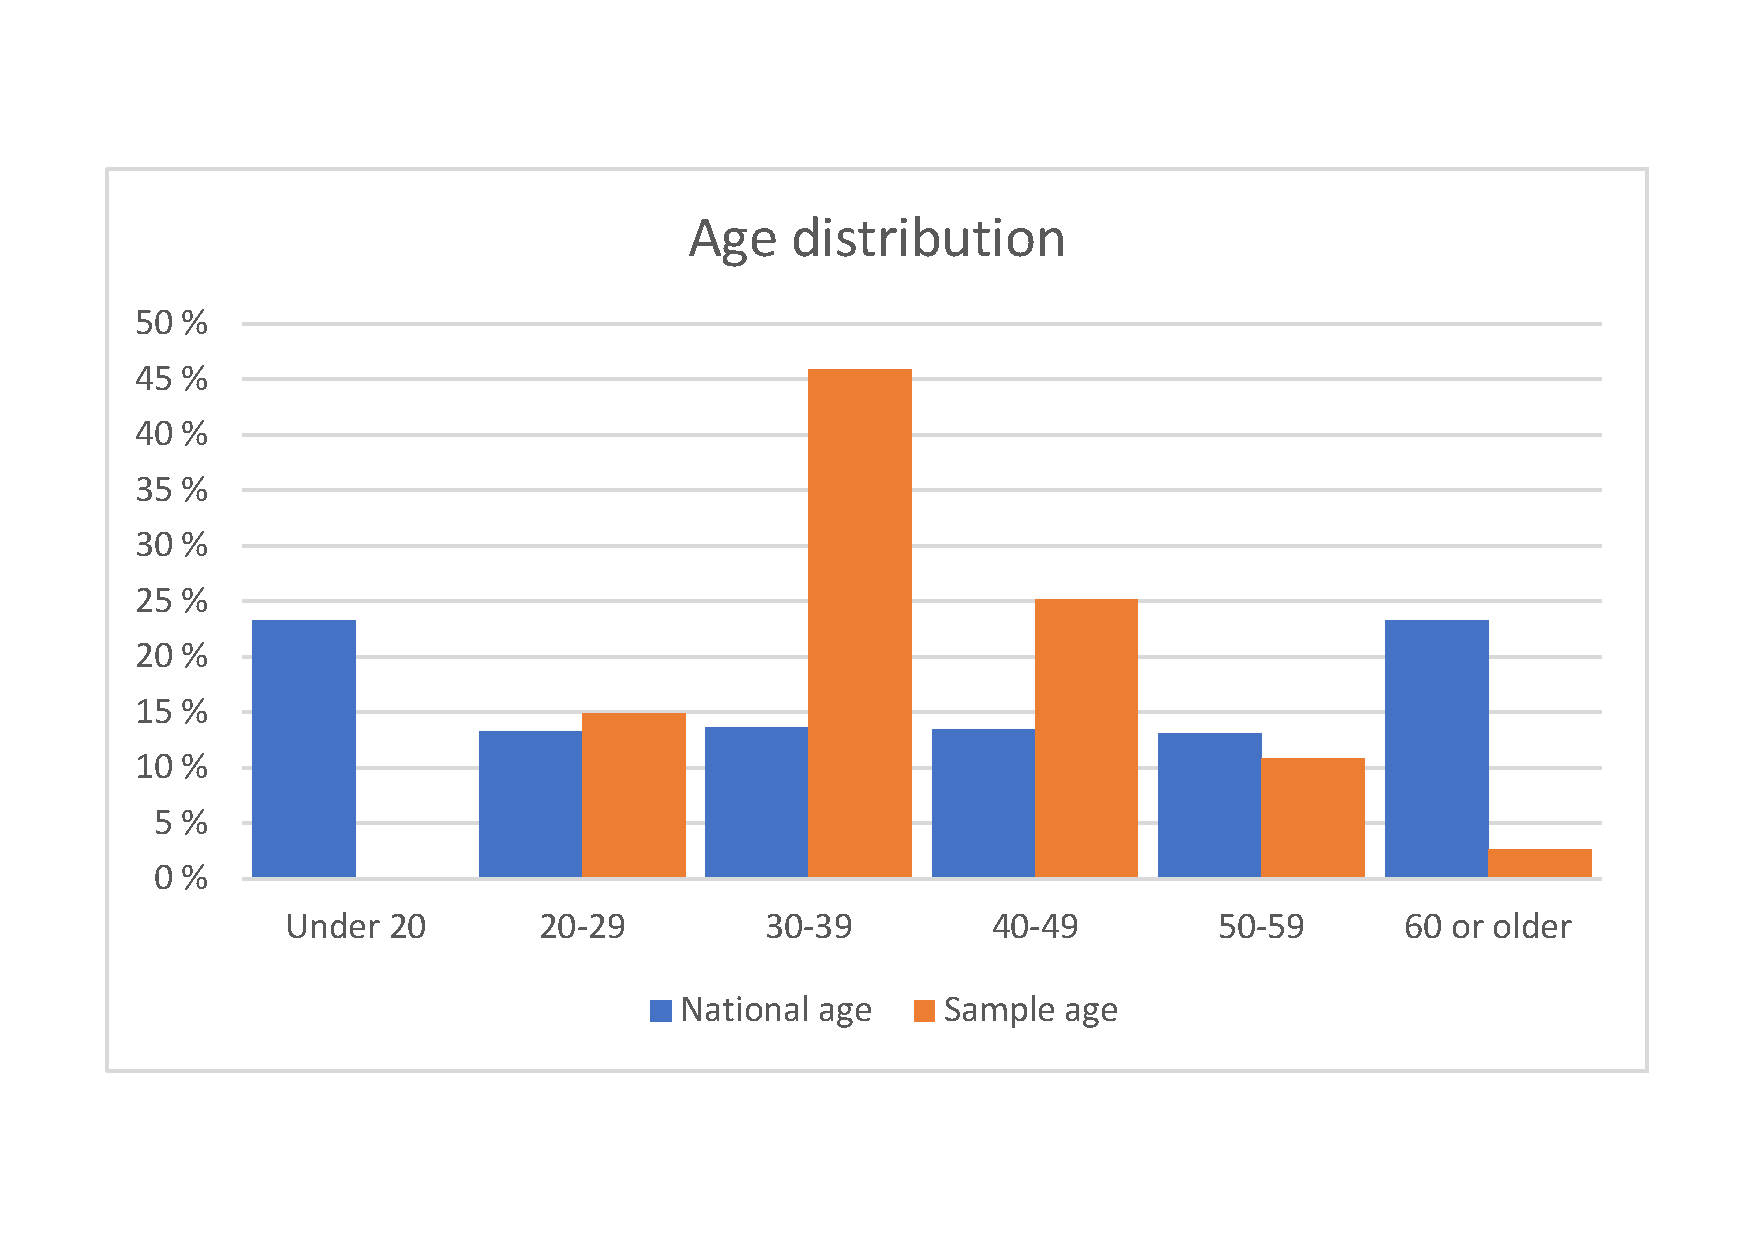
\includegraphics[scale=0.45]{figures/diagrams/age_ssb.pdf}
    \caption{Age distribution}
    \label{fig:age}
\end{figure}

As we can see from figure \ref{fig:age} above, we have a fairly middle-aged sample compared to the national population, which has a sizeable difference in younger and older people compared to my sample. 

Since the number of respondents being 60 or older in my sample only comprise 6 respondents, I will merge that category with 50-59 years going forward, resulting in a single category of 50 or older. This will result in the category comprising 30 respondents, which should be the minimum for further analysis between the groups. 

\subsection{Gender}
The gender distribution of my main sample is all men. There were also one respondent who did not want to specify, however there are no women in my sample. This makes it impossible to use in further analysis other than for sample description. This is obviously a huge deviation from the national average of approximately 50\% of each gender. 


\subsection{Highest completed education level}
None of the respondents answered that they had only primary school education or no education and only one person did not want to specify education level. 

\begin{figure}[H]
    \centering
    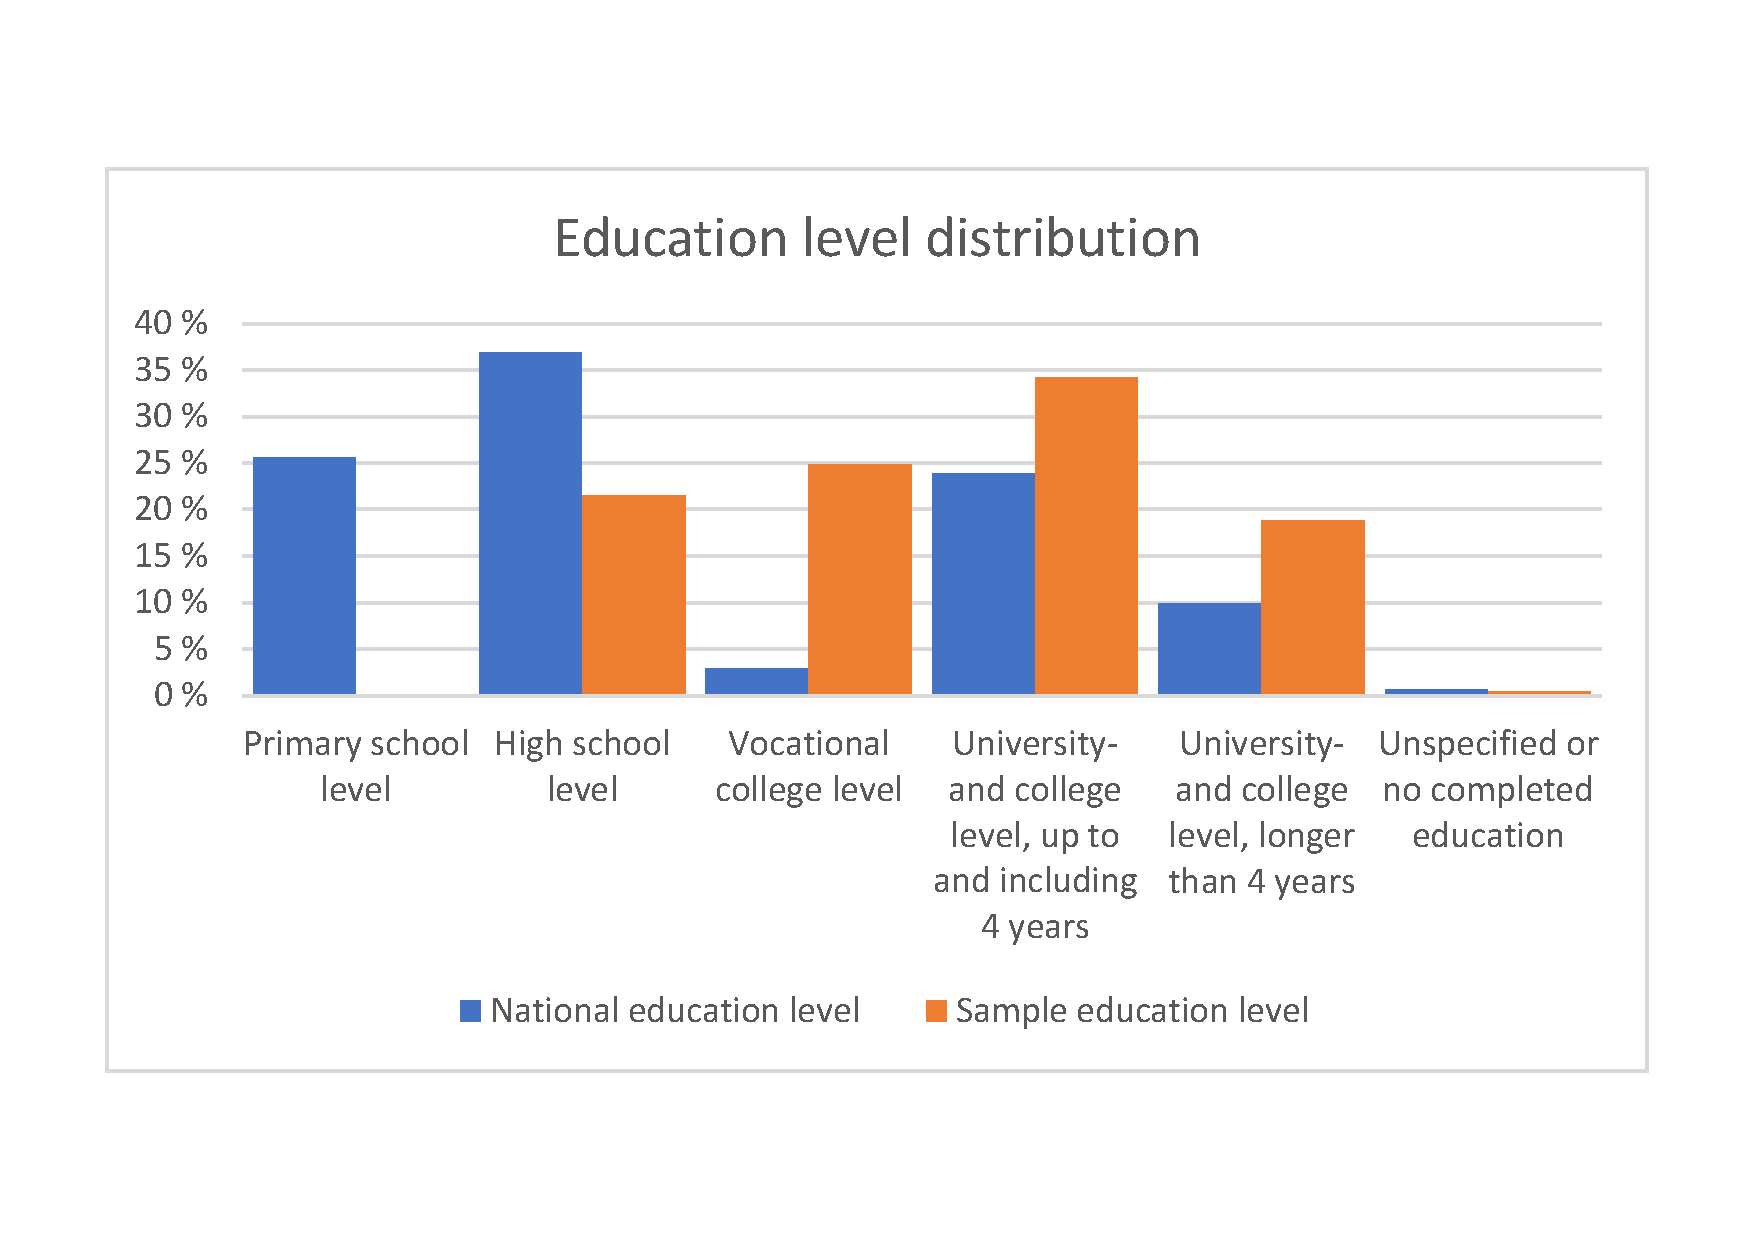
\includegraphics[scale=0.45]{figures/diagrams/education_ssb.pdf}
    \caption{Highest completed education level}
    \label{fig:education}
\end{figure}

From figure \ref{fig:education} above we can see that my sample contain a higher share of people with higher education. The most interesting fact is that there is a huge difference when it comes to people reporting to have a vocational education. 

\subsection{County}
There were two people who did not want to specify which county they lived in. The sample distribution in figure \ref{fig:county} below shows that it is very close to the national distribution. The only significant outlier is that my sample has a bit more people from Rogaland (14\%), compared to the national level (9\%).

\begin{figure}[H]
    \centering
    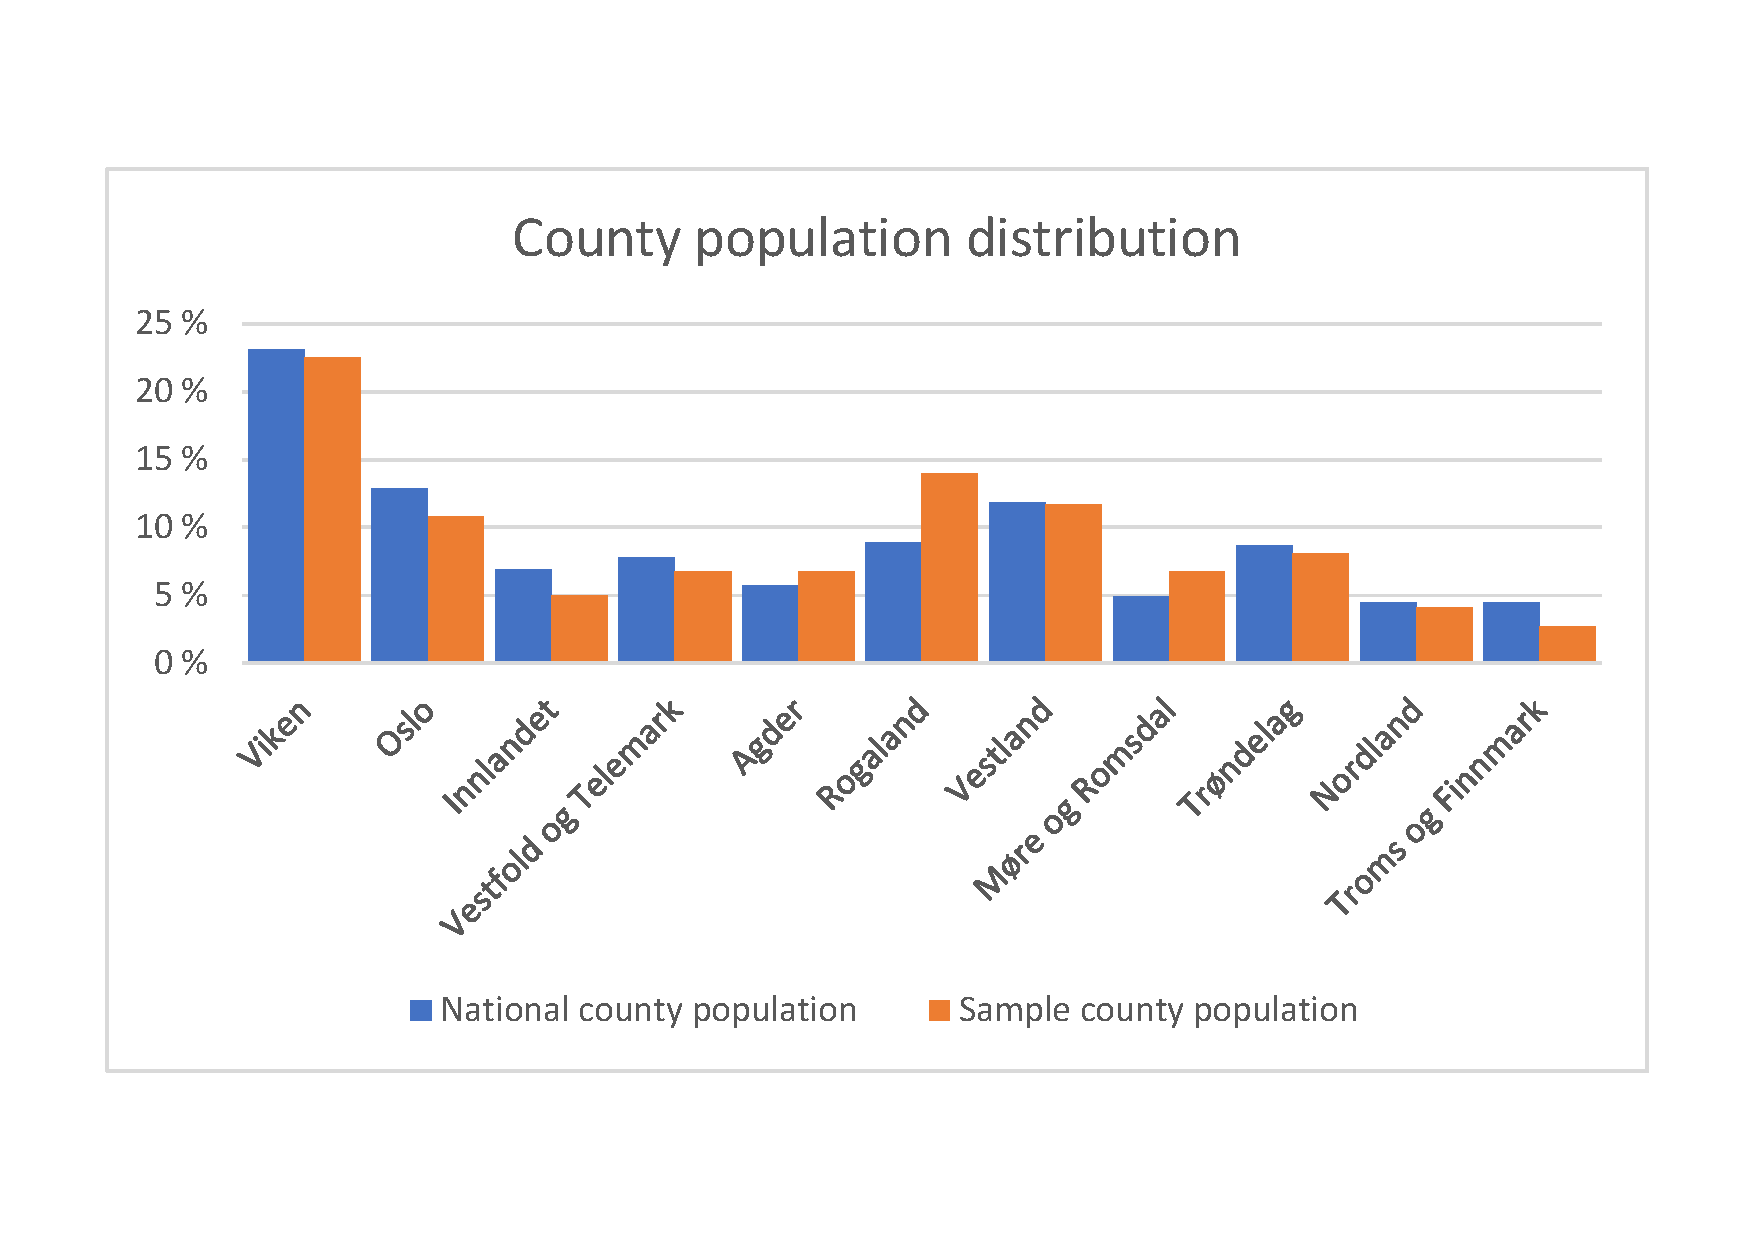
\includegraphics[scale=0.45]{figures/diagrams/county_ssb.pdf}
    \caption{County population distribution}
    \label{fig:county}
\end{figure}

It should be mentioned that most of the categories from my sample has less than 30 answers, which might impact the comparability of the numbers. For example, Troms og Finnmark only has 6 respondents in my sample, and Nordland has 9 respondents. At the other end of the spectrum lies Viken with 50 respondents and Rogaland with 31 respondents. 

\section{Background}

\subsection{How smart are the homes?}

\begin{table}[H]
\begin{tabular}{|l|c|c|c|c|c|c|}
\hline
\multicolumn{7}{|c|}{{\color[HTML]{010205} \textbf{Case summary}}}                                                                                                                                                                                                                                                                                                              \\ \hline
{\color[HTML]{264A60} }                                      & \multicolumn{6}{c|}{{\color[HTML]{264A60} Cases}}                                                                                                                                                                                                                                                                \\ \cline{2-7} 
{\color[HTML]{264A60} }                                      & \multicolumn{2}{c|}{{\color[HTML]{264A60} Valid}}                                                    & \multicolumn{2}{c|}{{\color[HTML]{264A60} Missing}}                                               & \multicolumn{2}{c|}{{\color[HTML]{264A60} Total}}                                                     \\ \cline{2-7} 
\multirow{-3}{*}{{\color[HTML]{264A60} }}                    & {\color[HTML]{264A60} N}                        & {\color[HTML]{264A60} Percent}                     & {\color[HTML]{264A60} N}                      & {\color[HTML]{264A60} Percent}                    & {\color[HTML]{264A60} N}                        & {\color[HTML]{264A60} Percent}                      \\ \hline
\cellcolor[HTML]{E0E0E0}{\color[HTML]{000000} Smart devices} & \multicolumn{1}{r|}{{\color[HTML]{010205} 219}} & \multicolumn{1}{r|}{{\color[HTML]{010205} 98.6\%}} & \multicolumn{1}{r|}{{\color[HTML]{010205} 3}} & \multicolumn{1}{r|}{{\color[HTML]{010205} 1.4\%}} & \multicolumn{1}{r|}{{\color[HTML]{010205} 222}} & \multicolumn{1}{r|}{{\color[HTML]{010205} 100.0\%}} \\ \hline
\end{tabular}
\end{table}

Out of the three that did not answer, two of them specified in freetext that they used a KNX system with control of heating, lighting, and ventilation, as well as motion sensors among other things. One respondent answered that they had no smart devices. 


\begin{table}[H]
\begin{tabular}{|l|l|r|r|r|}
\hline
\multicolumn{5}{|c|}{\textbf{Smart device types frequencies}}                                                                                                                                                                                                                                                                           \\ \hline
\multicolumn{2}{|l|}{}                                                                                                                           & \multicolumn{2}{c|}{{\color[HTML]{264A60} Responses}}                                               & \multicolumn{1}{c|}{{\color[HTML]{264A60} }}                                   \\ \cline{3-4}
\multicolumn{2}{|l|}{\multirow{-2}{*}{}}                                                                                                         & \multicolumn{1}{c|}{{\color[HTML]{264A60} N}} & \multicolumn{1}{c|}{{\color[HTML]{264A60} Percent}} & \multicolumn{1}{c|}{\multirow{-2}{*}{{\color[HTML]{264A60} Percent of Cases}}} \\ \hline
\cellcolor[HTML]{E0E0E0}{\color[HTML]{000000} }                                 & \cellcolor[HTML]{E0E0E0}{\color[HTML]{264A60} Voice assistant} & {\color[HTML]{010205} 155}                    & {\color[HTML]{010205} 6.7\%}                        & {\color[HTML]{010205} 70.8\%}                                                  \\ \cline{2-5} 
\cellcolor[HTML]{E0E0E0}{\color[HTML]{000000} }                                 & \cellcolor[HTML]{E0E0E0}{\color[HTML]{264A60} Speaker}         & {\color[HTML]{010205} 158}                    & {\color[HTML]{010205} 6.8\%}                        & {\color[HTML]{010205} 72.1\%}                                                  \\ \cline{2-5} 
\cellcolor[HTML]{E0E0E0}{\color[HTML]{000000} }                                 & \cellcolor[HTML]{E0E0E0}{\color[HTML]{264A60} Robot vaccum}    & {\color[HTML]{010205} 123}                    & {\color[HTML]{010205} 5.3\%}                        & {\color[HTML]{010205} 56.2\%}                                                  \\ \cline{2-5} 
\cellcolor[HTML]{E0E0E0}{\color[HTML]{000000} }                                 & \cellcolor[HTML]{E0E0E0}{\color[HTML]{264A60} Smart hub}       & {\color[HTML]{010205} 169}                    & {\color[HTML]{010205} 7.3\%}                        & {\color[HTML]{010205} 77.2\%}                                                  \\ \cline{2-5} 
\cellcolor[HTML]{E0E0E0}{\color[HTML]{000000} }                                 & \cellcolor[HTML]{E0E0E0}{\color[HTML]{264A60} Smart TV}        & {\color[HTML]{010205} 185}                    & {\color[HTML]{010205} 8.0\%}                        & {\color[HTML]{010205} 84.5\%}                                                  \\ \cline{2-5} 
\cellcolor[HTML]{E0E0E0}{\color[HTML]{000000} }                                 & \cellcolor[HTML]{E0E0E0}{\color[HTML]{264A60} Smart screen}    & {\color[HTML]{010205} 69}                     & {\color[HTML]{010205} 3.0\%}                        & {\color[HTML]{010205} 31.5\%}                                                  \\ \cline{2-5} 
\cellcolor[HTML]{E0E0E0}{\color[HTML]{000000} }                                 & \cellcolor[HTML]{E0E0E0}{\color[HTML]{264A60} Router}          & {\color[HTML]{010205} 143}                    & {\color[HTML]{010205} 6.2\%}                        & {\color[HTML]{010205} 65.3\%}                                                  \\ \cline{2-5} 
\cellcolor[HTML]{E0E0E0}{\color[HTML]{000000} }                                 & \cellcolor[HTML]{E0E0E0}{\color[HTML]{264A60} Door lock}       & {\color[HTML]{010205} 149}                    & {\color[HTML]{010205} 6.5\%}                        & {\color[HTML]{010205} 68.0\%}                                                  \\ \cline{2-5} 
\cellcolor[HTML]{E0E0E0}{\color[HTML]{000000} }                                 & \cellcolor[HTML]{E0E0E0}{\color[HTML]{264A60} Light bulbs}     & {\color[HTML]{010205} 163}                    & {\color[HTML]{010205} 7.1\%}                        & {\color[HTML]{010205} 74.4\%}                                                  \\ \cline{2-5} 
\cellcolor[HTML]{E0E0E0}{\color[HTML]{000000} }                                 & \cellcolor[HTML]{E0E0E0}{\color[HTML]{264A60} Smart dimmer}    & {\color[HTML]{010205} 181}                    & {\color[HTML]{010205} 7.8\%}                        & {\color[HTML]{010205} 82.6\%}                                                  \\ \cline{2-5} 
\cellcolor[HTML]{E0E0E0}{\color[HTML]{000000} }                                 & \cellcolor[HTML]{E0E0E0}{\color[HTML]{264A60} Smart switch}    & {\color[HTML]{010205} 177}                    & {\color[HTML]{010205} 7.7\%}                        & {\color[HTML]{010205} 80.8\%}                                                  \\ \cline{2-5} 
\cellcolor[HTML]{E0E0E0}{\color[HTML]{000000} }                                 & \cellcolor[HTML]{E0E0E0}{\color[HTML]{264A60} Kitchenware}     & {\color[HTML]{010205} 41}                     & {\color[HTML]{010205} 1.8\%}                        & {\color[HTML]{010205} 18.7\%}                                                  \\ \cline{2-5} 
\cellcolor[HTML]{E0E0E0}{\color[HTML]{000000} }                                 & \cellcolor[HTML]{E0E0E0}{\color[HTML]{264A60} Surveillance}    & {\color[HTML]{010205} 138}                    & {\color[HTML]{010205} 6.0\%}                        & {\color[HTML]{010205} 63.0\%}                                                  \\ \cline{2-5} 
\cellcolor[HTML]{E0E0E0}{\color[HTML]{000000} }                                 & \cellcolor[HTML]{E0E0E0}{\color[HTML]{264A60} Alarms}          & {\color[HTML]{010205} 111}                    & {\color[HTML]{010205} 4.8\%}                        & {\color[HTML]{010205} 50.7\%}                                                  \\ \cline{2-5} 
\cellcolor[HTML]{E0E0E0}{\color[HTML]{000000} }                                 & \cellcolor[HTML]{E0E0E0}{\color[HTML]{264A60} Montion sensors} & {\color[HTML]{010205} 177}                    & {\color[HTML]{010205} 7.7\%}                        & {\color[HTML]{010205} 80.8\%}                                                  \\ \cline{2-5} 
\multirow{-16}{*}{\cellcolor[HTML]{E0E0E0}{\color[HTML]{000000} Smart devices}} & \cellcolor[HTML]{E0E0E0}{\color[HTML]{264A60} Thermostat}      & {\color[HTML]{010205} 171}                    & {\color[HTML]{010205} 7.4\%}                        & {\color[HTML]{010205} 78.1\%}                                                  \\ \hline
\multicolumn{2}{|l|}{\cellcolor[HTML]{E0E0E0}{\color[HTML]{264A60} Total}}                                                                       & {\color[HTML]{010205} 2310}                   & {\color[HTML]{010205} 100.0\%}                      & {\color[HTML]{010205} 1054.8\%}                                                \\ \hline
\end{tabular}
\end{table}



\subsection{Household administrator}

\begin{figure}[H]
    \centering
    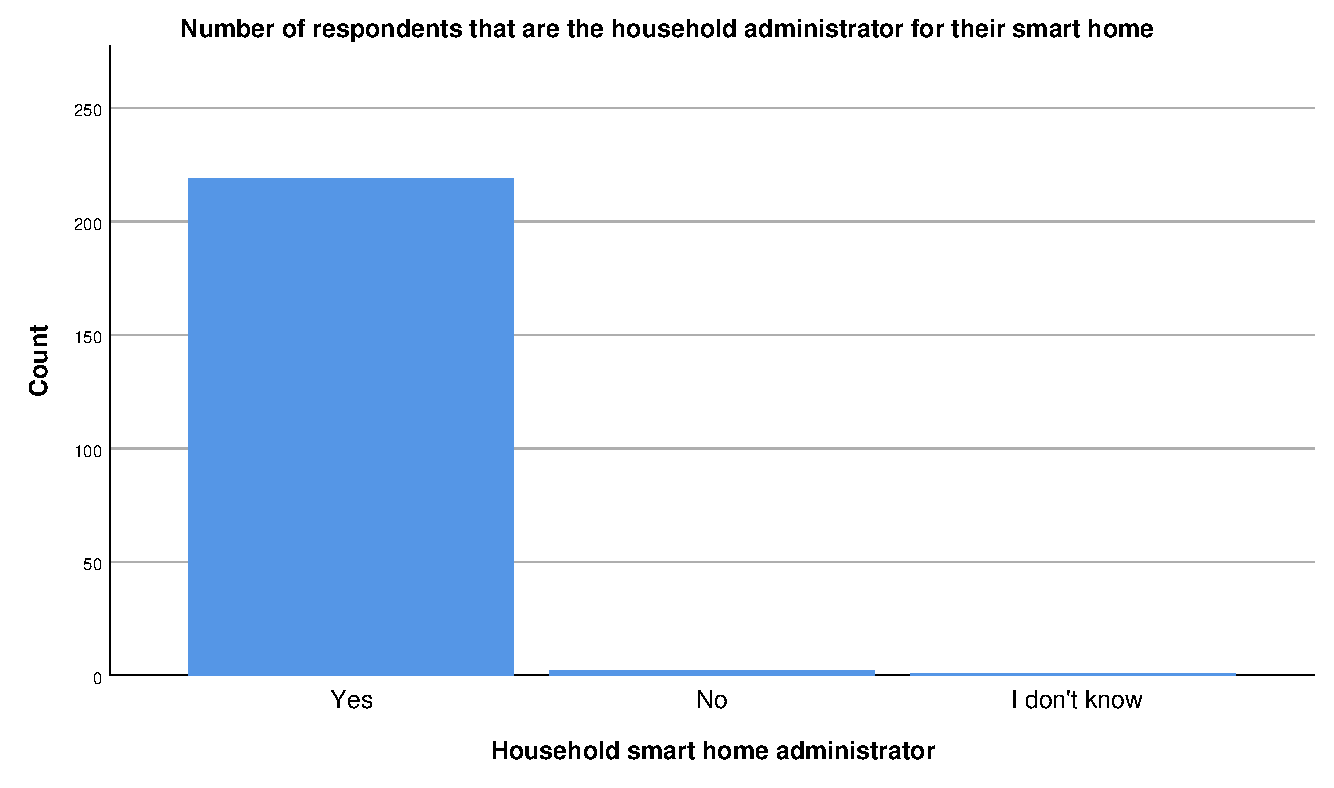
\includegraphics[scale=0.55]{figures/diagrams/administrator.pdf}
    \caption{Household administrators of their smart home}
    \label{fig:administrator}
\end{figure}

\subsection{Professional / hobby based background}

\begin{figure}[H]
    \centering
    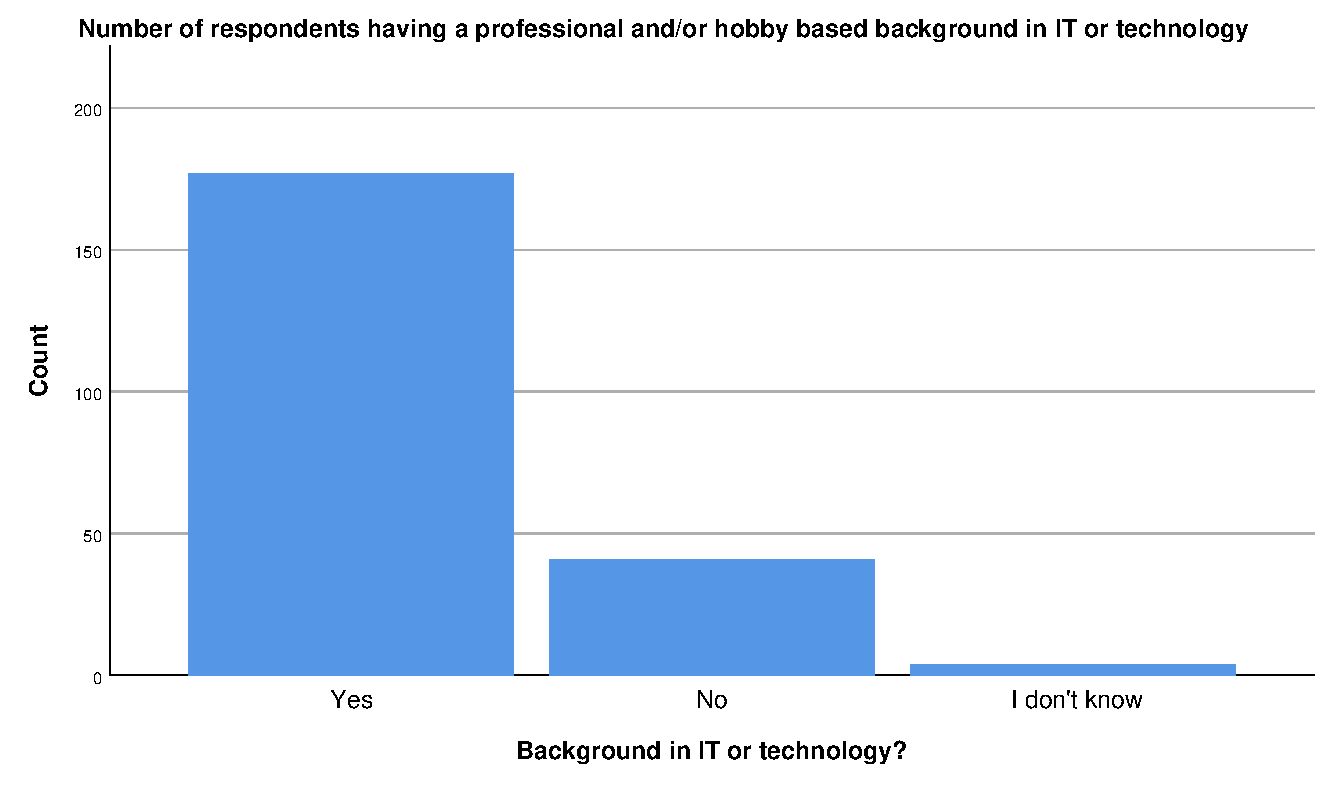
\includegraphics[scale=0.55]{figures/diagrams/background.pdf}
    \caption{The respondents background in IT or technology}
    \label{fig:background}
\end{figure}

\subsection{Knowledge of subjects}

\begin{figure}[H]
    \centering
    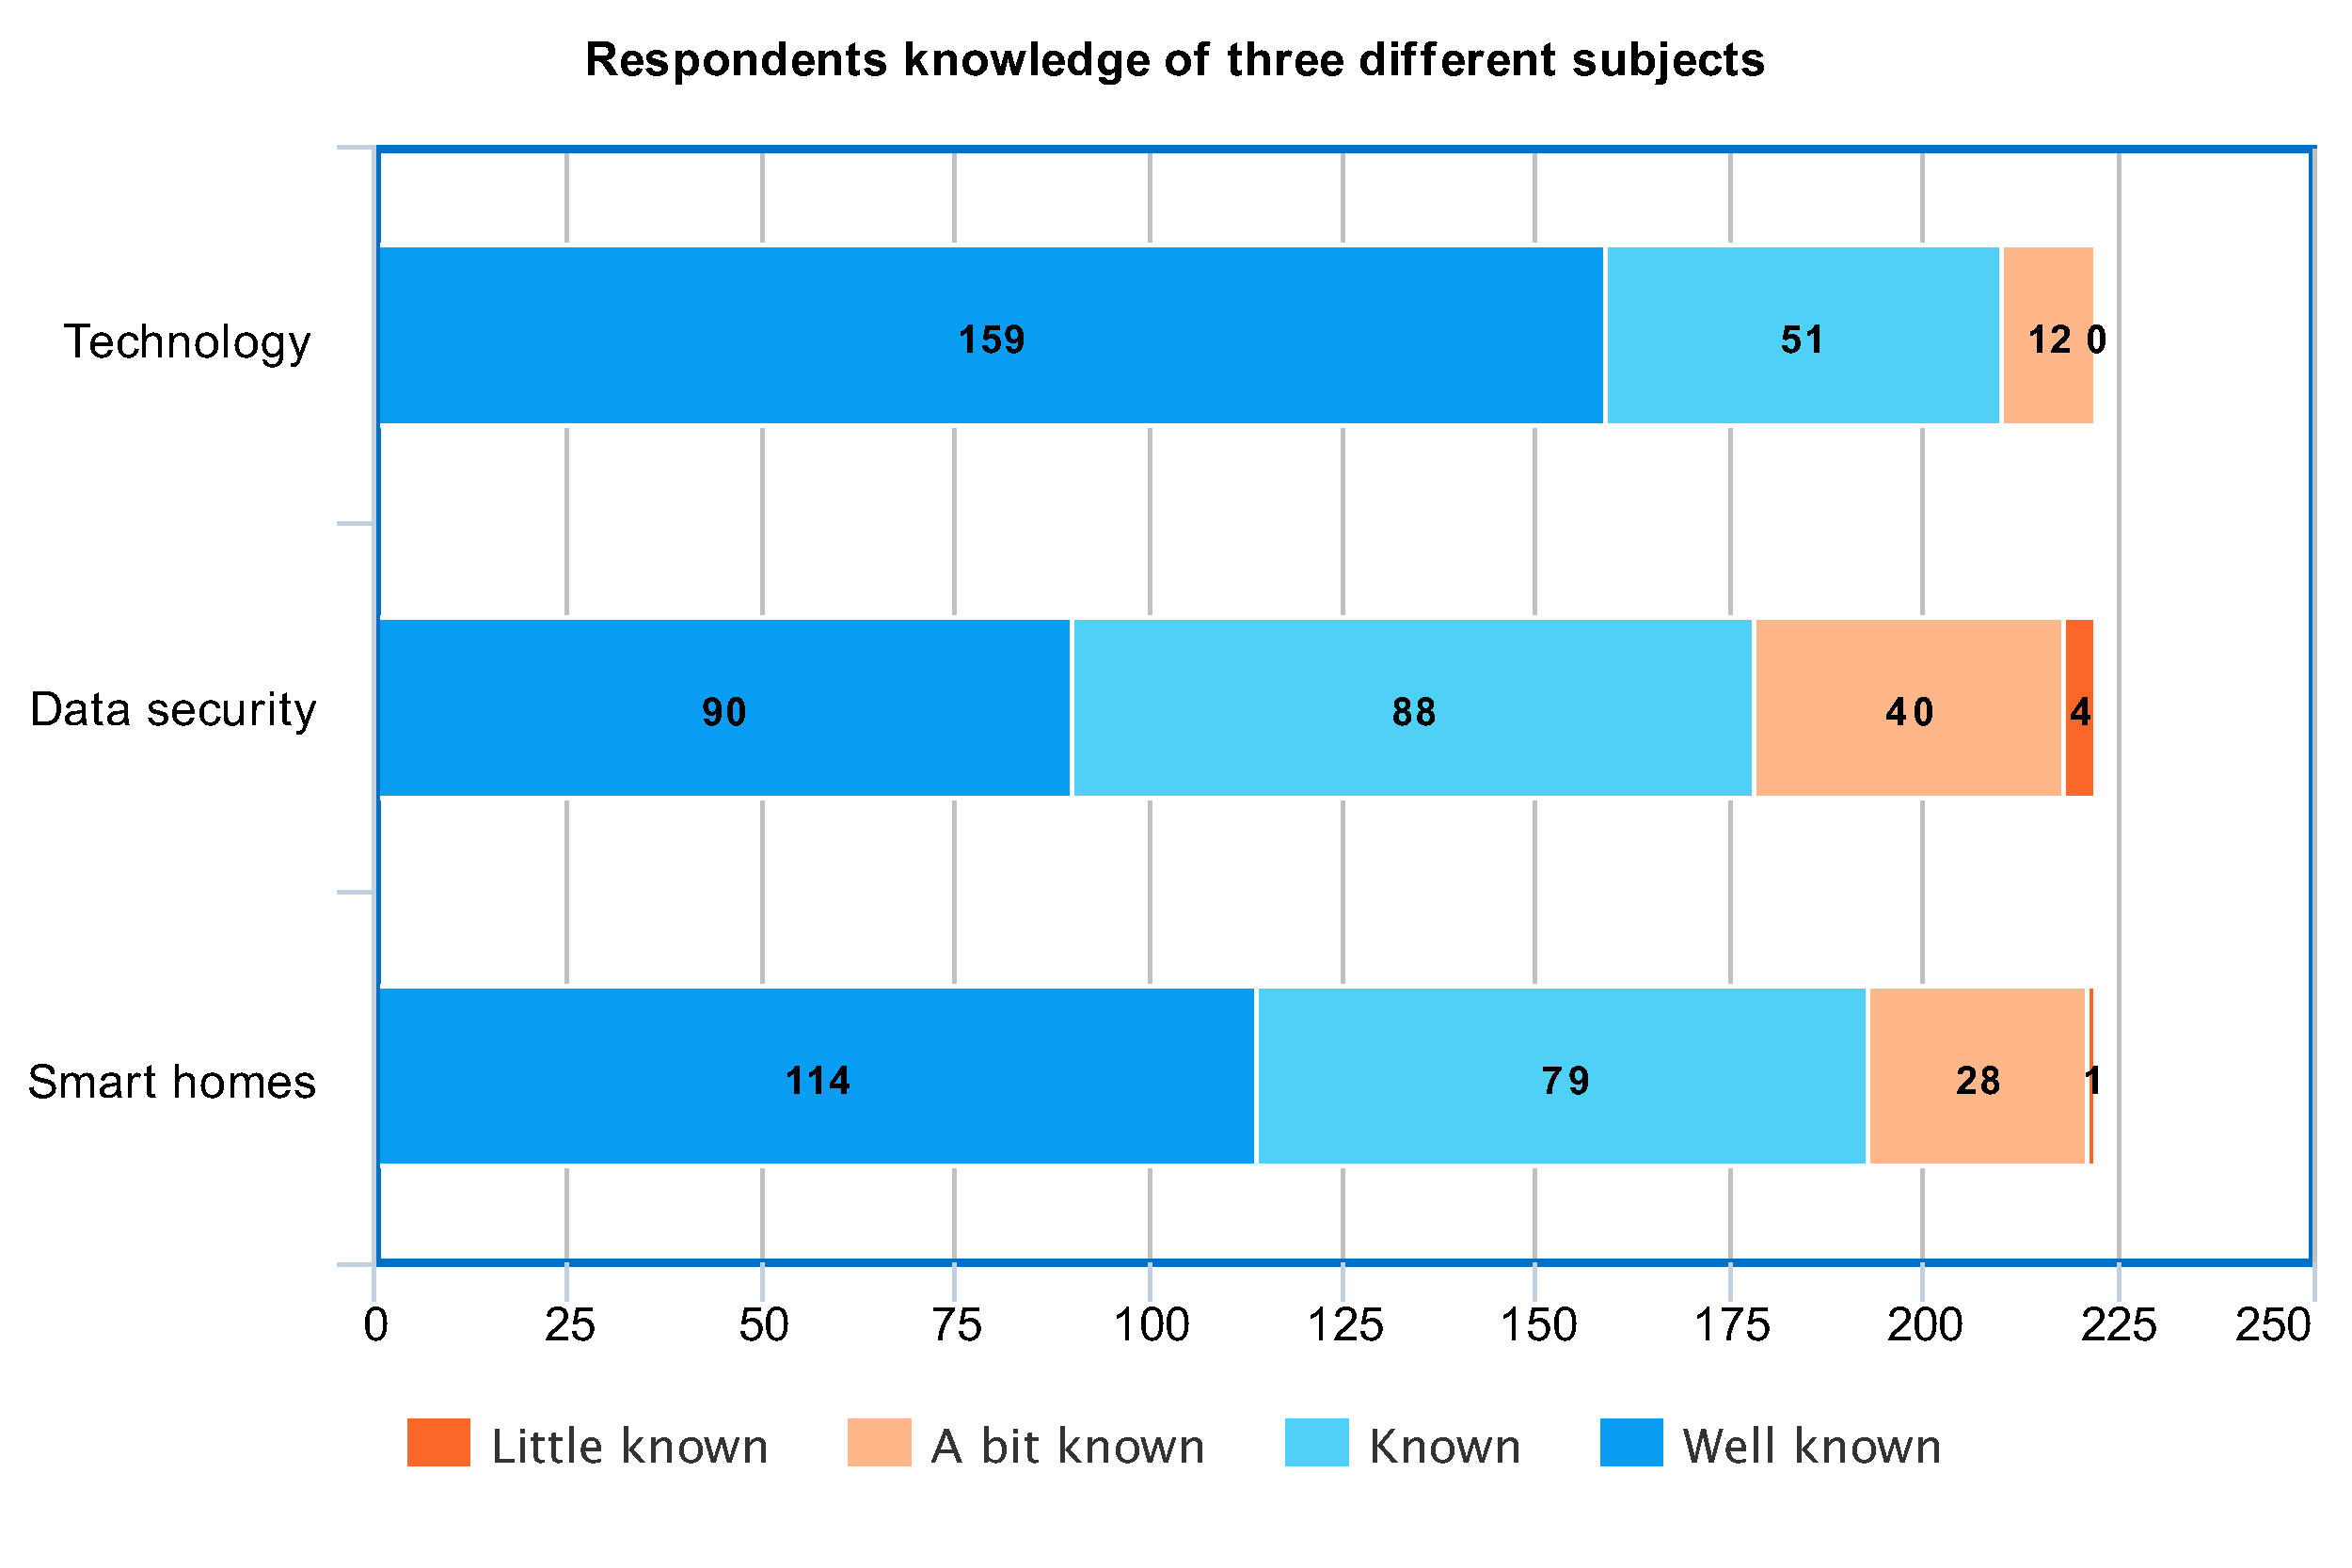
\includegraphics[scale=0.3]{figures/diagrams/knowledge.pdf}
    \caption{The respondents knowledge of three different subjects}
    \label{fig:knowledge}
\end{figure}


\section{Security awareness of the respondents}

\begin{figure}[H]
    \centering
    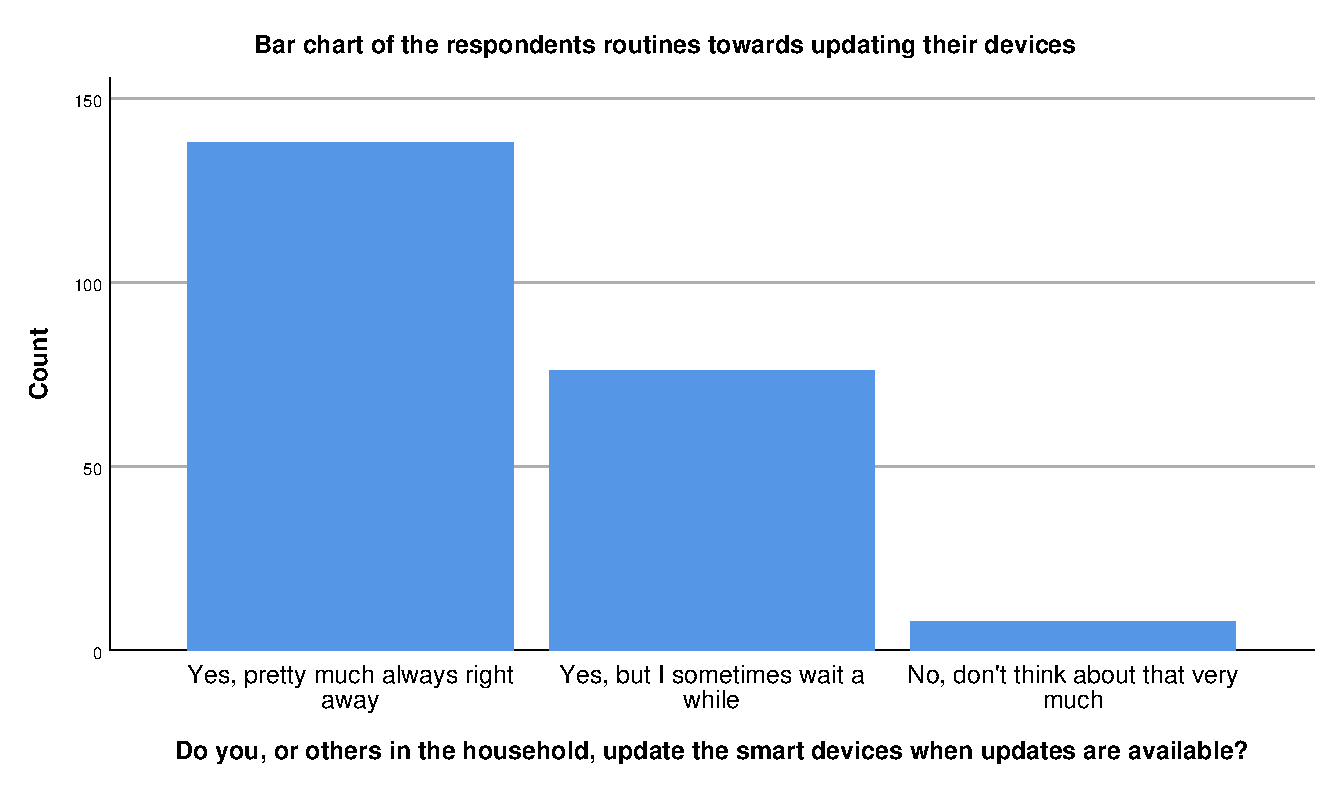
\includegraphics[scale=0.55]{figures/diagrams/update.pdf}
    \caption{The respondents routines towards updates their devices}
    \label{fig:update}
\end{figure}

\begin{figure}[H]
    \centering
    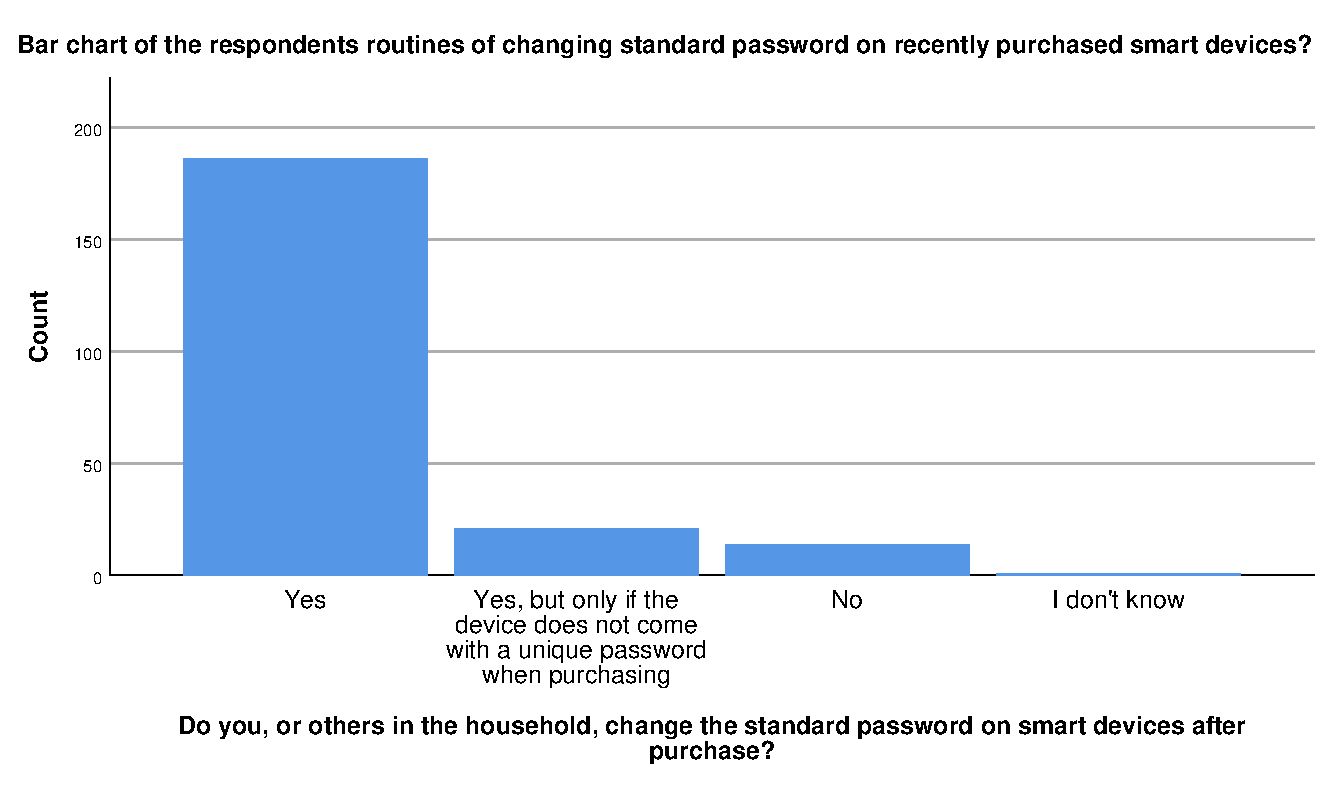
\includegraphics[scale=0.55]{figures/diagrams/standard_password.pdf}
    \caption{The respondents routines towards changing standard passwords}
    \label{fig:standard_password}
\end{figure}

\begin{figure}[H]
    \centering
    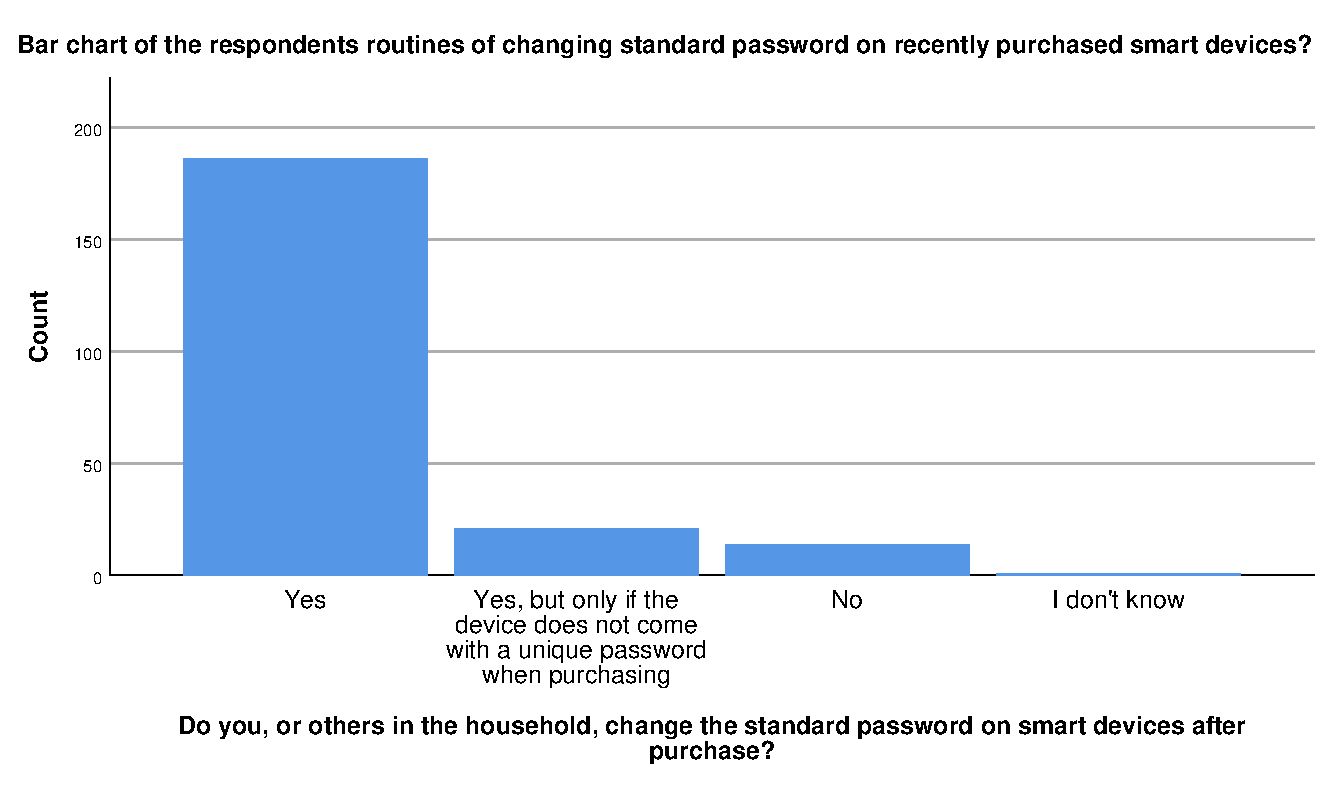
\includegraphics[scale=0.55]{figures/diagrams/standard_password.pdf}
    \caption{The respondents routines towards using password managers}
    \label{fig:standard_password}
\end{figure}

\begin{figure}[H]
    \centering
    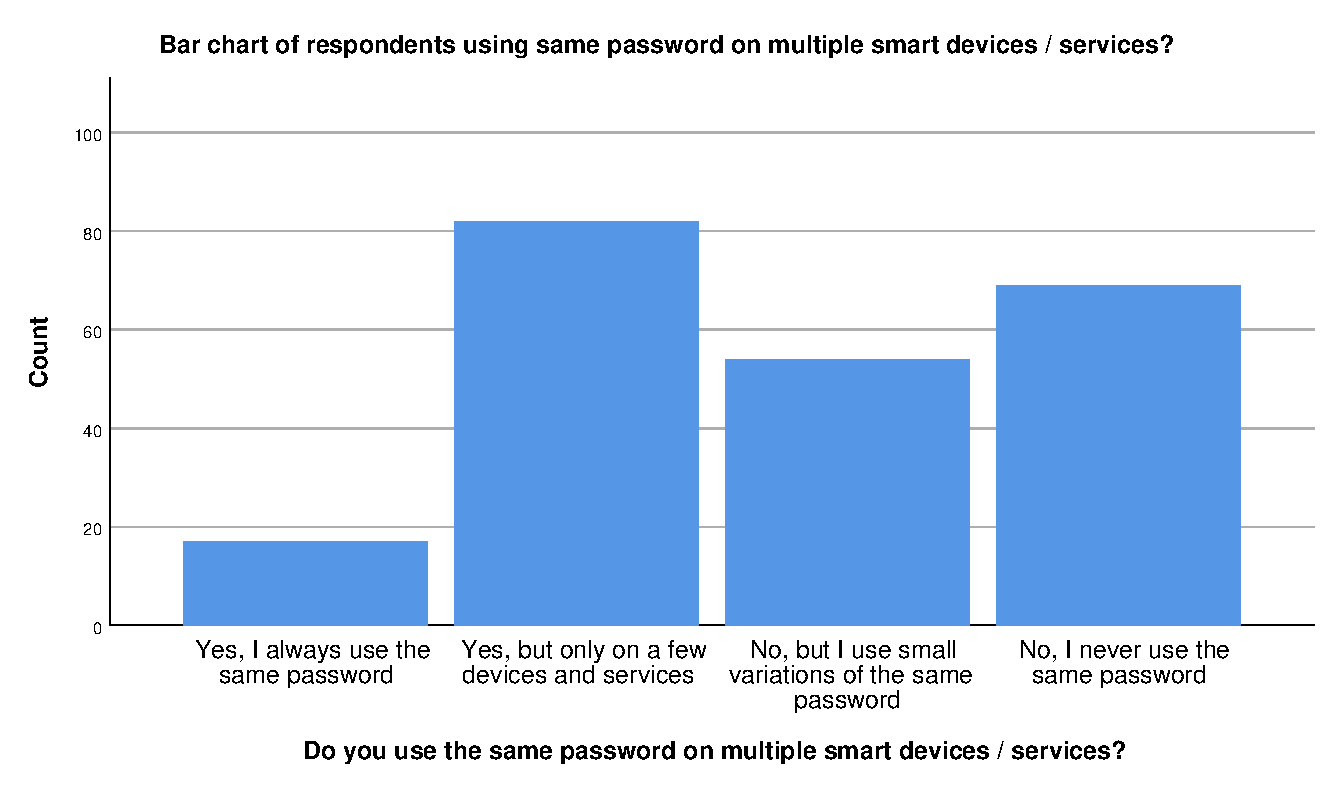
\includegraphics[scale=0.55]{figures/diagrams/password_reuse.pdf}
    \caption{The respondents routines towards using password on multiple devices/services}
    \label{fig:password_reuse}
\end{figure}

\begin{figure}[H]
    \centering
    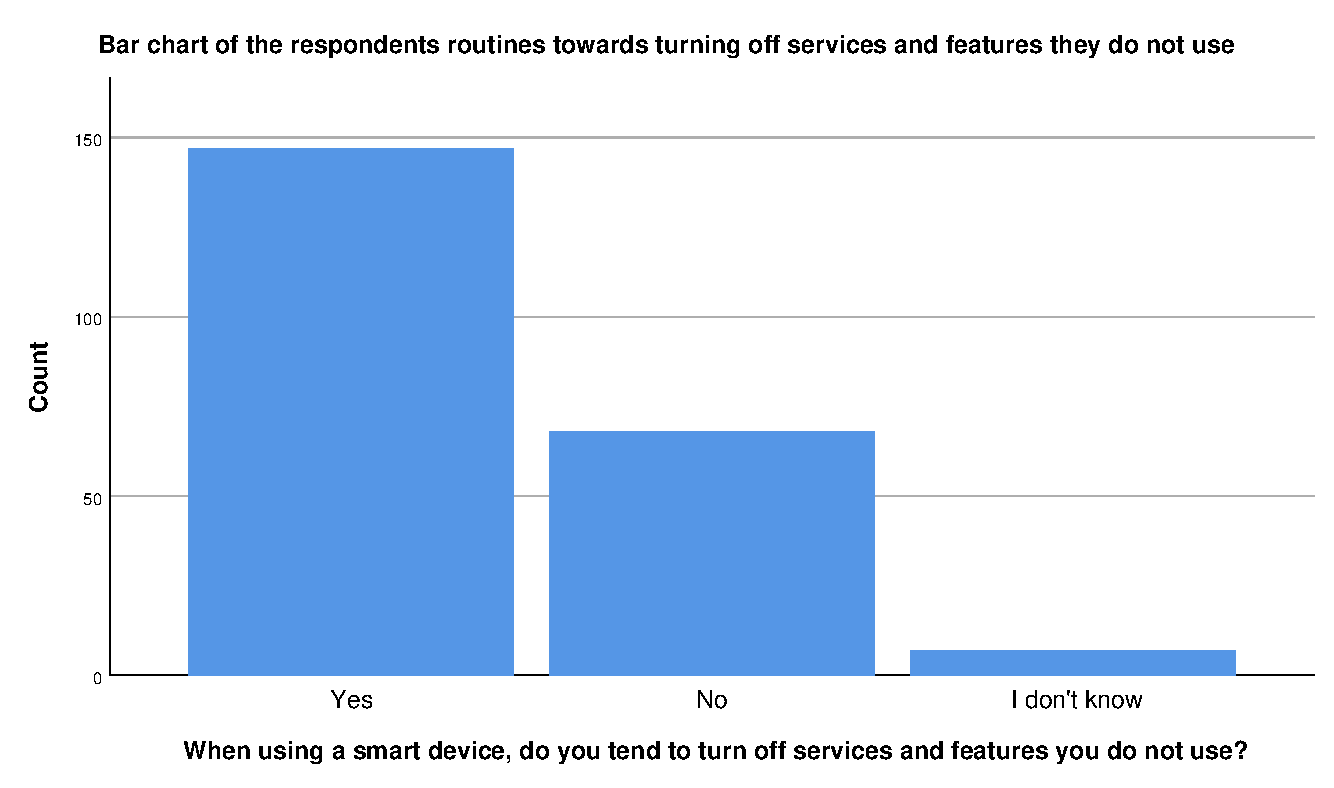
\includegraphics[scale=0.55]{figures/diagrams/turn_off_features.pdf}
    \caption{The respondents routines towards turning off features and services they do not use}
    \label{fig:turn_off_features}
\end{figure}

\begin{figure}[H]
    \centering
    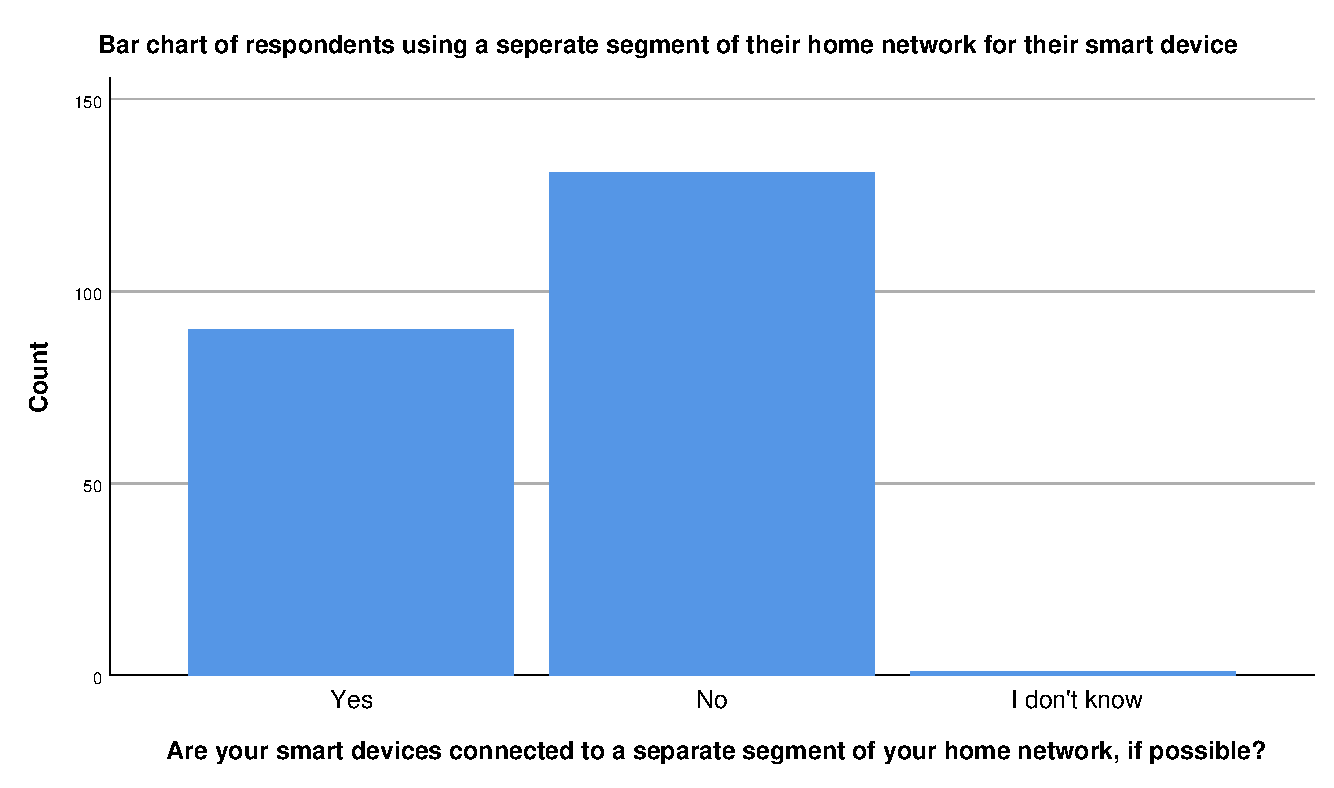
\includegraphics[scale=0.55]{figures/diagrams/separat_segment.pdf}
    \caption{The respondents routines towards connecting smart devices to a separate home network segment}
    \label{fig:separat_segment}
\end{figure}

\begin{figure}[H]
    \centering
    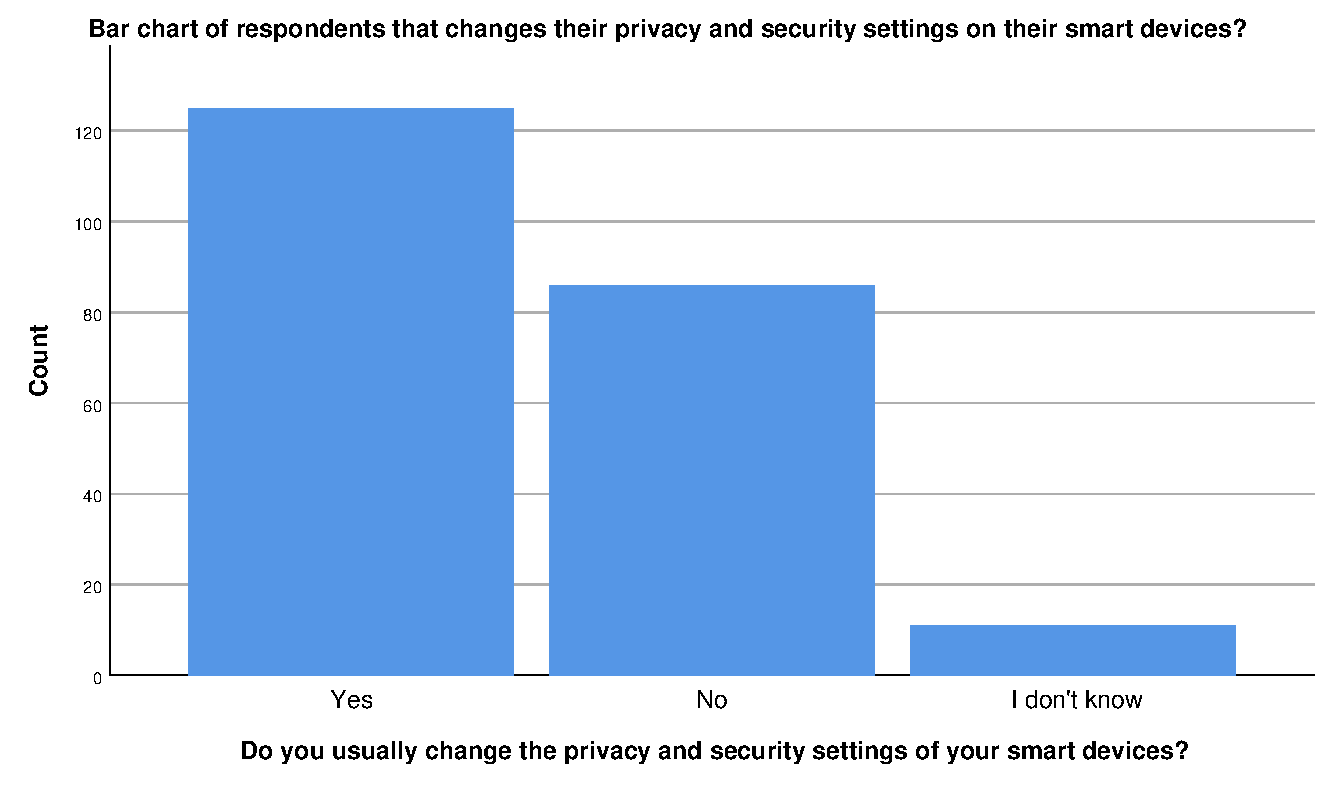
\includegraphics[scale=0.55]{figures/diagrams/settings.pdf}
    \caption{The respondents routines towards changing their security and privacy settings}
    \label{fig:settings}
\end{figure}

\begin{figure}[H]
    \centering
    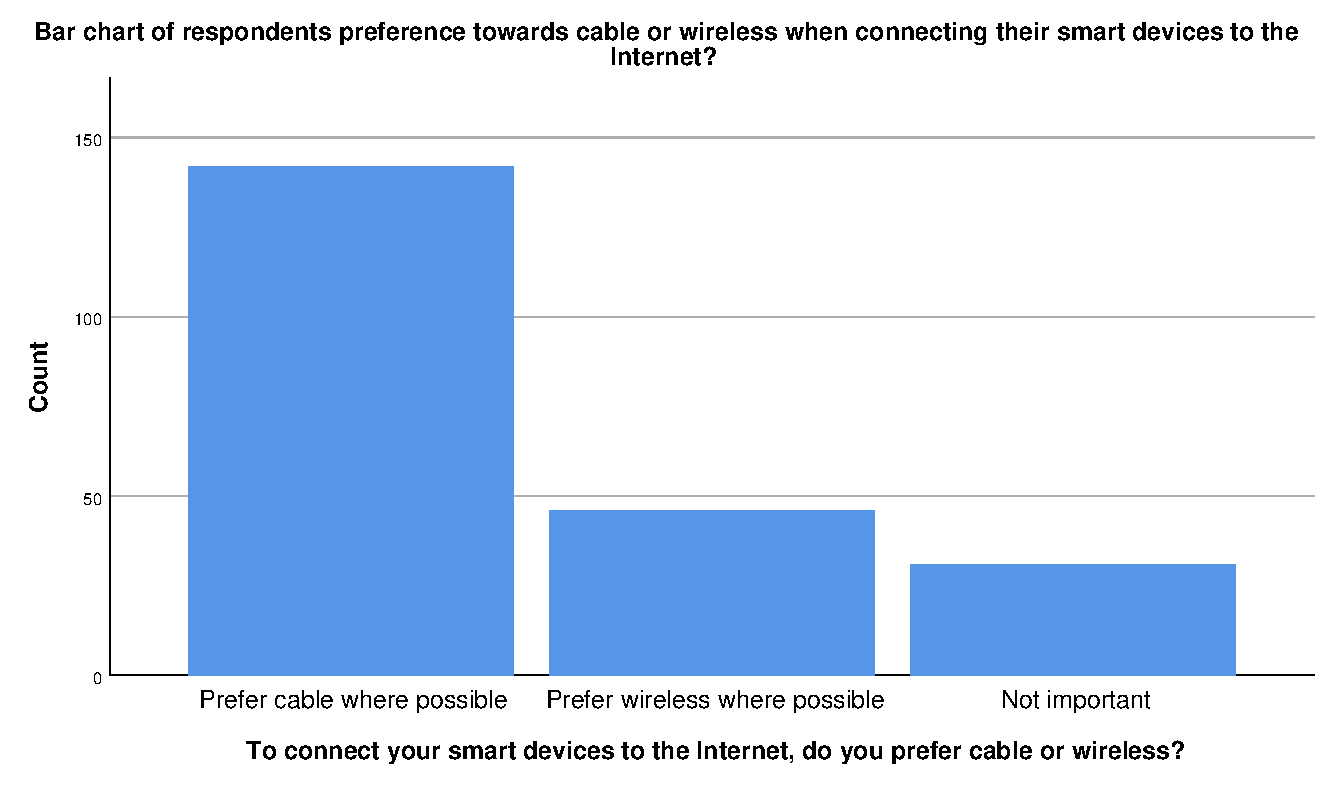
\includegraphics[scale=0.55]{figures/diagrams/connect_internet.pdf}
    \caption{The respondents preference for cable or wireless when connecting their smart devices to the Internet}
    \label{fig:connect_internet}
\end{figure}

\begin{figure}[H]
    \centering
    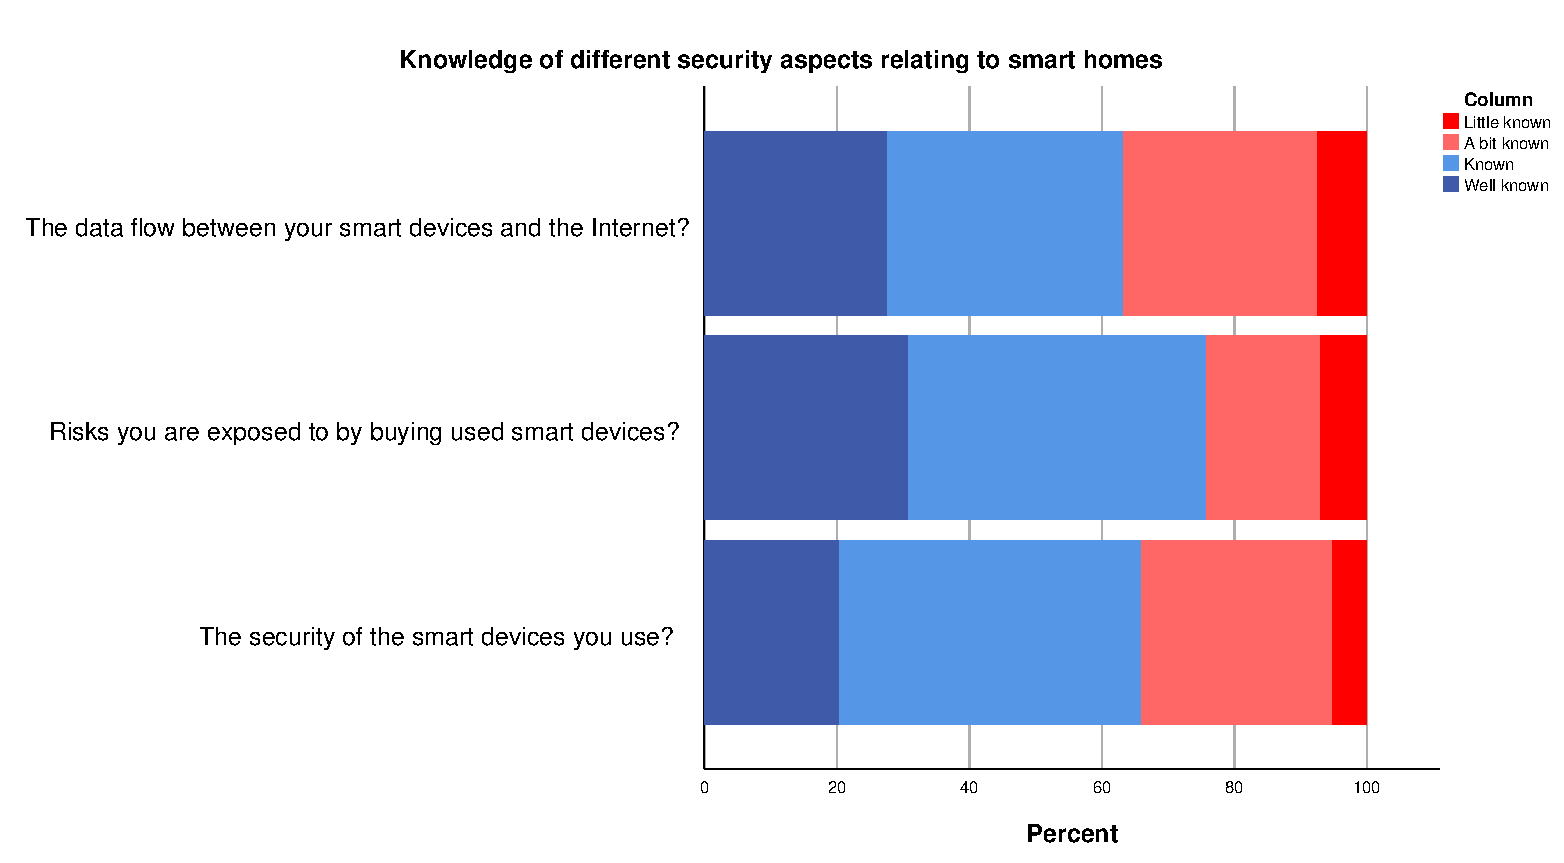
\includegraphics[scale=0.45]{figures/diagrams/knowledge_security.pdf}
    \caption{Knowledge of different security aspects relating to smart homes}
    \label{fig:knowledge_security}
\end{figure}

\section{Risk perceptions of the respondents}

\begin{figure}[H]
    \centering
    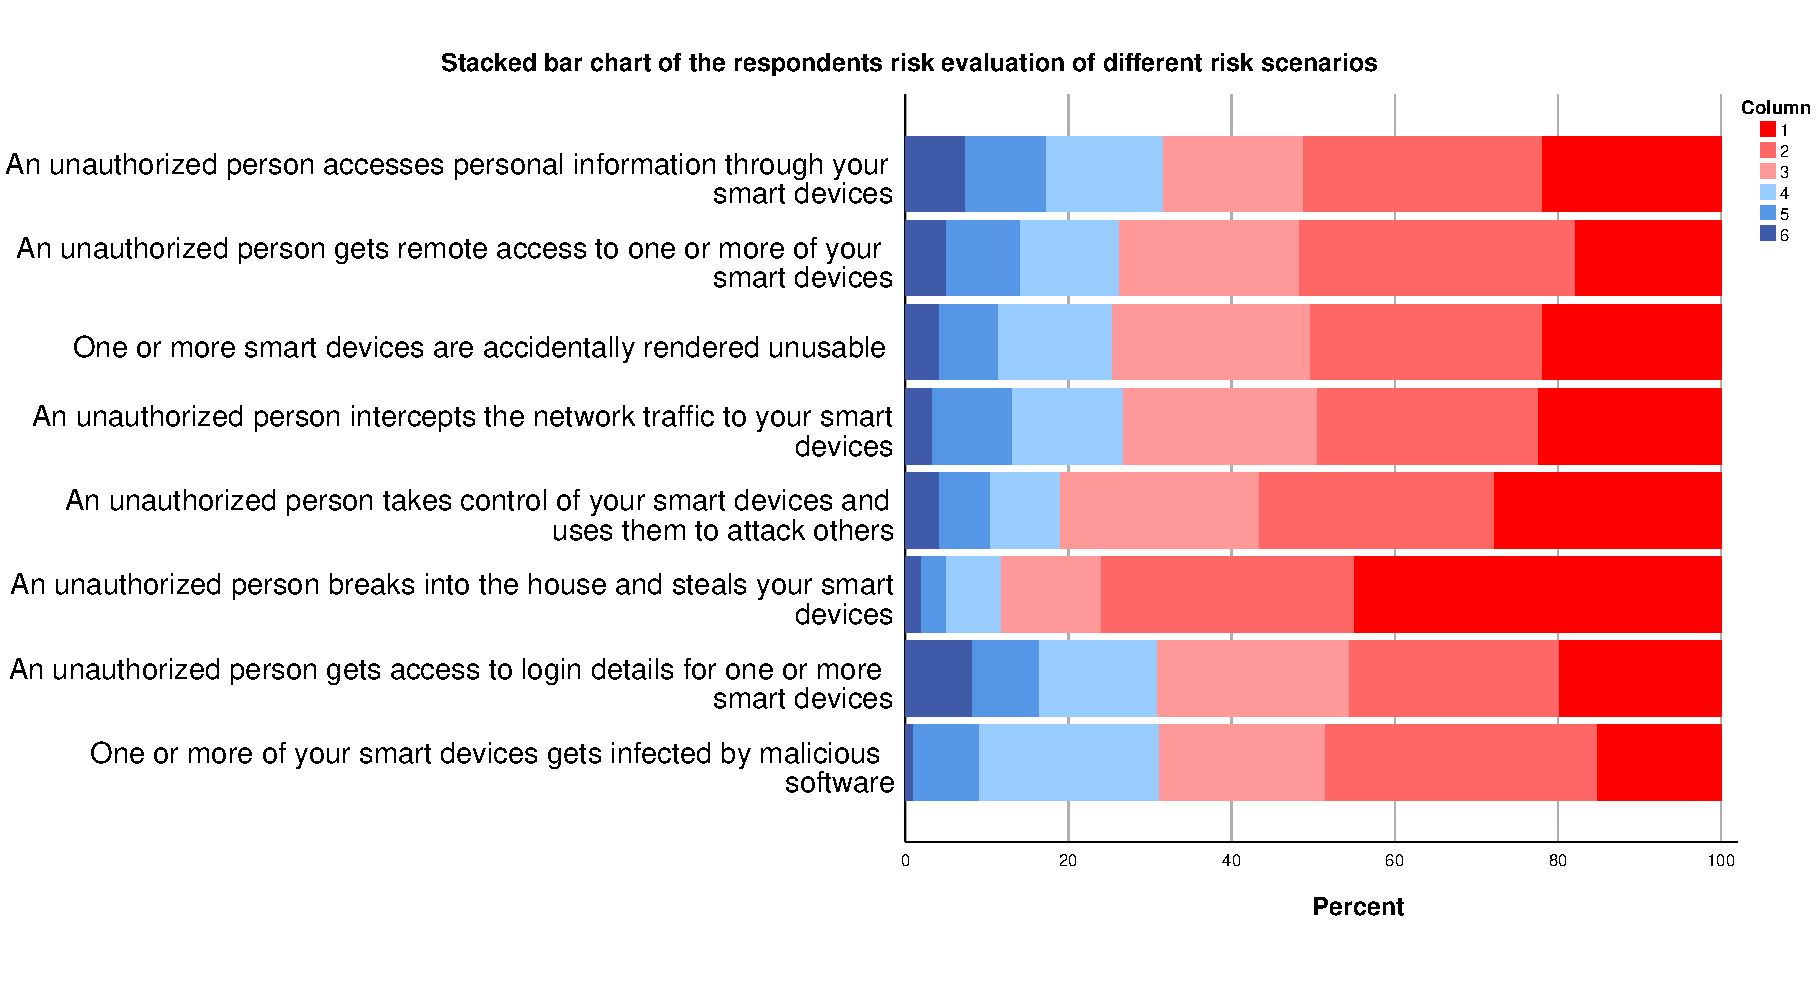
\includegraphics[scale=0.4]{figures/diagrams/risk_perception.pdf}
    \caption{Respondents risk evaluation of different risk scenarios}
    \label{fig:risk perception}
\end{figure}